\documentclass[screen]{beamer}
\usepackage{listings}
\usepackage{color}
\usepackage{bold-extra}
\usepackage{wasysym}
\usepackage{beamerthemesplit}
\usepackage{graphicx}
\usetheme{default}

\definecolor{Brown}{cmyk}{0,0.81,1,0.60}
\definecolor{OliveGreen}{cmyk}{0.64,0,0.95,0.40}
\definecolor{CadetBlue}{cmyk}{0.62,0.57,0.23,0}
\renewcommand{\ttdefault}{pcr}
\newcommand{\badgood}[2]{%
	\begin{columns}%
		\column{.5\textwidth}%
		\begin{alertblock}{Bad}%
			#1%
		\end{alertblock}%
		\column{.5\textwidth}%
		\begin{exampleblock}{Good}%
			#2%
		\end{exampleblock}%
	\end{columns}%
}%
\title{Initial Examples}
\author{Andrey Breslav}
\institute{ITMO University, St. Petersburg / University of Tartu}
\date{Oct. 30, 2009}

\begin{document}

\lstset{
  language=Java,
  basicstyle=\ttfamily\normalsize,
  keywordstyle=\bfseries\color{Brown},
  commentstyle=\color{OliveGreen},
  stringstyle=\color[rgb]{0,0,1},
  tabsize=4
}

\begin{frame}[t,fragile]
%%%%%%%%%%%%%%%%%%%%%%%%%%%%%%%%%%%%%%%%%%%%%%%%%%%%%%%%%%%%%%%%%%%%%%%%%%%%%%%%%%%%%%%%%%%%%%%%%%%%%%%%%%%%%%
\frametitle{What does this program print?}%
\begin{block}{Attempt 1}
\begin{lstlisting}
public class Rec {
private static int f(int 
x){
if(x<2){    return 
	1;
}return f(x- 
1)+f(x-2
);}
public static void main(
String[] args) {
System.out.println(f(5));}}
\end{lstlisting}%
\end{block}
%%%%%%%%%%%%%%%%%%%%%%%%%%%%%%%%%%%%%%%%%%%%%%%%%%%%%%%%%%%%%%%%%%%%%%%%%%%%%%%%%%%%%%%%%%%%%%%%%%%%%%%%%%%%%%
\end{frame}

\begin{frame}[t,fragile]
%%%%%%%%%%%%%%%%%%%%%%%%%%%%%%%%%%%%%%%%%%%%%%%%%%%%%%%%%%%%%%%%%%%%%%%%%%%%%%%%%%%%%%%%%%%%%%%%%%%%%%%%%%%%%%
\frametitle{What does this program print?}%
%
\begin{block}{Attempt 2: A hint\ldots}%
\begin{lstlisting}
public class Rec {
    private static int f(int x) {
		if (x < 2) {
			return 1;
		}
		return f(x - 1) + f(x - 2);
	}

	public static void main(String[] args) {
		System.out.println(f(5));
	}
}
\end{lstlisting}%
\end{block}%
%%%%%%%%%%%%%%%%%%%%%%%%%%%%%%%%%%%%%%%%%%%%%%%%%%%%%%%%%%%%%%%%%%%%%%%%%%%%%%%%%%%%%%%%%%%%%%%%%%%%%%%%%%%%%%
\end{frame}

\begin{frame}[c,fragile]
%%%%%%%%%%%%%%%%%%%%%%%%%%%%%%%%%%%%%%%%%%%%%%%%%%%%%%%%%%%%%%%%%%%%%%%%%%%%%%%%%%%%%%%%%%%%%%%%%%%%%%%%%%%%%%
\frametitle{What does this class do?}%
%
\begin{block}{Attempt 1}%
\begin{lstlisting}
public static final class Oc {
	private final Object[] e 
					= new Object[1000000];
	private int pe = -1;
	private int po = 0;

	public void a(Object x) {
		e[po++] = x;
	}

	public Object b() {
		return e[pe++];
	}
}
\end{lstlisting}%
\end{block}%

%%%%%%%%%%%%%%%%%%%%%%%%%%%%%%%%%%%%%%%%%%%%%%%%%%%%%%%%%%%%%%%%%%%%%%%%%%%%%%%%%%%%%%%%%%%%%%%%%%%%%%%%%%%%%%
\end{frame}

\begin{frame}[c,fragile]
%%%%%%%%%%%%%%%%%%%%%%%%%%%%%%%%%%%%%%%%%%%%%%%%%%%%%%%%%%%%%%%%%%%%%%%%%%%%%%%%%%%%%%%%%%%%%%%%%%%%%%%%%%%%%%
\frametitle{What does this class do?}%
%
\begin{block}{Attempt 2: A hint\ldots}
\begin{lstlisting}
public static final class Queue {
	private final Object[] myValues 
					= new Object[BIG_VALUE];
	private int myHead = -1;
	private int myTail = 0;
	
	public void enqueue(Object x) {
		myValues[myTail++] = x;
	}
	
	public Object dequeue() {
		return myValues[myHead++];
	}
}
\end{lstlisting}%
\end{block}
%%%%%%%%%%%%%%%%%%%%%%%%%%%%%%%%%%%%%%%%%%%%%%%%%%%%%%%%%%%%%%%%%%%%%%%%%%%%%%%%%%%%%%%%%%%%%%%%%%%%%%%%%%%%%%
\end{frame}

\begin{frame}[c,fragile]
%%%%%%%%%%%%%%%%%%%%%%%%%%%%%%%%%%%%%%%%%%%%%%%%%%%%%%%%%%%%%%%%%%%%%%%%%%%%%%%%%%%%%%%%%%%%%%%%%%%%%%%%%%%%%%
\frametitle{A bug fixed}%
%
\begin{block}{class Queue}
\begin{lstlisting}
	private int myHead = -1;
	private int myTail = 0;
	
	public void enqueue(Object x) {
		myValues[myTail] = x;
		myTail++;
	}
	
	public Object dequeue() {
		myHead++;
		return myValues[myHead];
	}
\end{lstlisting}%
\end{block}
%%%%%%%%%%%%%%%%%%%%%%%%%%%%%%%%%%%%%%%%%%%%%%%%%%%%%%%%%%%%%%%%%%%%%%%%%%%%%%%%%%%%%%%%%%%%%%%%%%%%%%%%%%%%%%
\end{frame}

\begin{frame}[t,fragile]
%%%%%%%%%%%%%%%%%%%%%%%%%%%%%%%%%%%%%%%%%%%%%%%%%%%%%%%%%%%%%%%%%%%%%%%%%%%%%%%%%%%%%%%%%%%%%%%%%%%%%%%%%%%%%%
\frametitle{What does this function do?}%
%
\begin{block}{A humble two-line function \smiley}
\begin{lstlisting}
boolean p(int x) {
	int y = x * (030 >> 4 << 030);
	return y == 0;
}
\end{lstlisting}%		
\end{block}

\begin{block}{Hints}<2->
	\begin{itemize}
		\item \texttt{a << s = a * $\mathtt{2^s}$} --- bitwise shift left
		\item \texttt{a >> s = a / $\mathtt{2^s}$} --- bitwise shift right
		\item \texttt{0x<DIGITS>} --- hexadecimal number
		\item \texttt{0<DIGITS>} --- octal number
	\end{itemize}
\end{block}
%%%%%%%%%%%%%%%%%%%%%%%%%%%%%%%%%%%%%%%%%%%%%%%%%%%%%%%%%%%%%%%%%%%%%%%%%%%%%%%%%%%%%%%%%%%%%%%%%%%%%%%%%%%%%%
\end{frame}

\begin{frame}[fragile]
%%%%%%%%%%%%%%%%%%%%%%%%%%%%%%%%%%%%%%%%%%%%%%%%%%%%%%%%%%%%%%%%%%%%%%%%%%%%%%%%%%%%%%%%%%%%%%%%%%%%%%%%%%%%%%
\frametitle{What we have (hopefully) learned so far}%
%
\begin{block}{Example 1: Fibonacci numbers}<2->
	Format your programs properly!
\end{block}
\begin{block}{Example 2: Queue}<3->
	Give understandable names to program elements!\\
	\begin{itemize}
		\item<4-> A good program does not demand comments other than JavaDoc for interfaces.
	\end{itemize}
\end{block}
\begin{block}{Example 3: Divisibility by 256}<5->
	Do not outsmart yourself!\\
	\uncover<6->{Use understandable code constructs.}
\end{block}
%%%%%%%%%%%%%%%%%%%%%%%%%%%%%%%%%%%%%%%%%%%%%%%%%%%%%%%%%%%%%%%%%%%%%%%%%%%%%%%%%%%%%%%%%%%%%%%%%%%%%%%%%%%%%%
\end{frame}

\title{Coding Conventions for Java}
\frame{\titlepage}

\begin{frame}[fragile]
%%%%%%%%%%%%%%%%%%%%%%%%%%%%%%%%%%%%%%%%%%%%%%%%%%%%%%%%%%%%%%%%%%%%%%%%%%%%%%%%%%%%%%%%%%%%%%%%%%%%%%%%%%%%%%
\frametitle{Exercise 1}%
%
\begin{itemize}[<+->]
	\item Groups: 4 people each
	\item Time: 10 minutes
	\item Task: come up with 2 rules (conventions)
		\begin{itemize}
			\item Clear formulations
			\item Clear explanations
		\end{itemize}
\end{itemize}
%%%%%%%%%%%%%%%%%%%%%%%%%%%%%%%%%%%%%%%%%%%%%%%%%%%%%%%%%%%%%%%%%%%%%%%%%%%%%%%%%%%%%%%%%%%%%%%%%%%%%%%%%%%%%%
\end{frame}

\begin{frame}[fragile]
%%%%%%%%%%%%%%%%%%%%%%%%%%%%%%%%%%%%%%%%%%%%%%%%%%%%%%%%%%%%%%%%%%%%%%%%%%%%%%%%%%%%%%%%%%%%%%%%%%%%%%%%%%%%%%
\frametitle{Sun's CCJ}%
%
\begin{block}
	{``Code Conventions for Java\texttrademark{} Programming Language''}
	http://java.sun.com/docs/codeconv/
	\begin{itemize}
		\item A ``standard'' provided by the Sun Microsystems 
		\item Reflects the opinion of the creators of the language
		\item Adopted by many projects
	\end{itemize}
\end{block}
%%%%%%%%%%%%%%%%%%%%%%%%%%%%%%%%%%%%%%%%%%%%%%%%%%%%%%%%%%%%%%%%%%%%%%%%%%%%%%%%%%%%%%%%%%%%%%%%%%%%%%%%%%%%%%
\end{frame}

%%%%%%%%%%%%%%%%%%%%%%%%%%%%%%
% Conventions
%%%%%%%%%%%%%%%%%%%%%%%%%%%%%%

%%%%%%%%%%%%%%%%
%%%%%%%%%%%%%%%% Naming
%%%%%%%%%%%%%%%%
\begin{frame}[fragile]
%%%%%%%%%%%%%%%%%%%%%%%%%%%%%%%%%%%%%%%%%%%%%%%%%%%%%%%%%%%%%%%%%%%%%%%%%%%%%%%%%%%%%%%%%%%%%%%%%%%%%%%%%%%%%%
\frametitle{Naming Conventions: Types and Methods}%
%
\begin{block}{Classes and Interfaces}
	\begin{itemize}
		\item Class name is most likely a noun phrase
		\item Written in CamelCase
			\begin{itemize}
				\item MyFavouriteClass
			\end{itemize}
		\item{} [Not in CCJ]: Interface names are prefixed with ``I'': IModel
	\end{itemize}
\end{block}
\begin{block}{Methods}
	\begin{itemize}
		\item Method name is most likely a verb phrase
		\item Starts with a lower case letter, then --- CamelCase
			\begin{itemize}
				\item doTheJob()
			\end{itemize}
		\item{} Common prefixes ``get'', ``is'', ``set''
	\end{itemize}
\end{block}
%%%%%%%%%%%%%%%%%%%%%%%%%%%%%%%%%%%%%%%%%%%%%%%%%%%%%%%%%%%%%%%%%%%%%%%%%%%%%%%%%%%%%%%%%%%%%%%%%%%%%%%%%%%%%%
\end{frame}

\begin{frame}[fragile]
%%%%%%%%%%%%%%%%%%%%%%%%%%%%%%%%%%%%%%%%%%%%%%%%%%%%%%%%%%%%%%%%%%%%%%%%%%%%%%%%%%%%%%%%%%%%%%%%%%%%%%%%%%%%%%
\frametitle{Naming Conventions: Variables and Constants}%
%
\begin{block}{Variables: fields, local variables, parameters}
	\begin{itemize}
		\item Starts with a lower case letter, then --- CamelCase
			\begin{itemize}
				\item counter, firstOccurrence
			\end{itemize}
		\item Names should never start with ``\$'' or ``\_''
		\item{} [Not in CCJ]: field names are prefixed with ``my''
	\end{itemize}
\end{block}
\begin{block}{Constants: {\bf static final}, normally {\bf public}}
	\begin{itemize}
		\item Uppercase letters, words separated by underscores ``\_''
			\begin{itemize}
				\item THE\_CONSTANT
			\end{itemize}
	\end{itemize}
\end{block}
%%%%%%%%%%%%%%%%%%%%%%%%%%%%%%%%%%%%%%%%%%%%%%%%%%%%%%%%%%%%%%%%%%%%%%%%%%%%%%%%%%%%%%%%%%%%%%%%%%%%%%%%%%%%%%
\end{frame}

\begin{frame}[fragile]
%%%%%%%%%%%%%%%%%%%%%%%%%%%%%%%%%%%%%%%%%%%%%%%%%%%%%%%%%%%%%%%%%%%%%%%%%%%%%%%%%%%%%%%%%%%%%%%%%%%%%%%%%%%%%%
\frametitle{Naming Conventions: Packages}%
%
\begin{block}{Packages}
	\begin{itemize}
		\item Only lowercase ASCII letters
		\item Starts with a unique domain name (reversed)
			\begin{itemize}
				\item org.eclipse.emf.ecore
			\end{itemize}
	\end{itemize}
\end{block}
%%%%%%%%%%%%%%%%%%%%%%%%%%%%%%%%%%%%%%%%%%%%%%%%%%%%%%%%%%%%%%%%%%%%%%%%%%%%%%%%%%%%%%%%%%%%%%%%%%%%%%%%%%%%%%
\end{frame}
%%%%%%%%%%%%%%%%
%%%%%%%%%%%%%%%% Declaration order
%%%%%%%%%%%%%%%%
\begin{frame}[fragile]
%%%%%%%%%%%%%%%%%%%%%%%%%%%%%%%%%%%%%%%%%%%%%%%%%%%%%%%%%%%%%%%%%%%%%%%%%%%%%%%%%%%%%%%%%%%%%%%%%%%%%%%%%%%%%%
\frametitle{Declaration Order: Elements of a Class}%
%
\begin{block}{Only one top-level class should be declared in a file}
\end{block}
\begin{block}{Order of elements in a class}
	\begin{enumerate}
		\item Nested classes
		\item Static fields
		\item Static methods
		\item Constructors
		\item Instance fields
		\item Instance methods
	\end{enumerate}
\end{block}
%%%%%%%%%%%%%%%%%%%%%%%%%%%%%%%%%%%%%%%%%%%%%%%%%%%%%%%%%%%%%%%%%%%%%%%%%%%%%%%%%%%%%%%%%%%%%%%%%%%%%%%%%%%%%%
\end{frame}

\begin{frame}[fragile]
%%%%%%%%%%%%%%%%%%%%%%%%%%%%%%%%%%%%%%%%%%%%%%%%%%%%%%%%%%%%%%%%%%%%%%%%%%%%%%%%%%%%%%%%%%%%%%%%%%%%%%%%%%%%%%
\frametitle{Declaration Order: Inside a Method}%
%
\begin{block}{Only one variable per line (applies also to fields)}
	\badgood{
		\lstinline!int a = 0, b = 3;!\\
		$\;$\\
	}{
		\lstinline!int a = 0;!\\
		\lstinline!int b = 3;!\\
	}
\end{block}
\begin{block}{Variables are initialized upon declaration (if possible)}
	\badgood{
		\lstinline!int a;!
	}{
		\lstinline!int a = 0;!
	}
\end{block}
\begin{block}{[Not in CCJ]: Variables are defined as close to their usage as possible}
	\uncover<2>{
		\alert{Actually CCJ recommends the opposite}
	}
\end{block}
%%%%%%%%%%%%%%%%%%%%%%%%%%%%%%%%%%%%%%%%%%%%%%%%%%%%%%%%%%%%%%%%%%%%%%%%%%%%%%%%%%%%%%%%%%%%%%%%%%%%%%%%%%%%%%
\end{frame}

\begin{frame}[fragile]
%%%%%%%%%%%%%%%%%%%%%%%%%%%%%%%%%%%%%%%%%%%%%%%%%%%%%%%%%%%%%%%%%%%%%%%%%%%%%%%%%%%%%%%%%%%%%%%%%%%%%%%%%%%%%%
\frametitle{Declaration Order: Variable Declaration Example}%
\begin{columns}
	\column{.5\textwidth}
%\badgood{
\begin{alertblock}{Bad}
\begin{lstlisting}
int a = 0;
int b = 5;
while (b > 0) {
    a = b * b;
    if (a > 10) {
        c++;
    }
}
\end{lstlisting}
\end{alertblock}
%}{
	\column{.5\textwidth}
\begin{exampleblock}{Good}
\begin{lstlisting}
int b = 5;
while (b > 0) {
    int a = b * b;
    if (a > 10) {
        c++;
    }
}
\end{lstlisting}
$\,$\\
$\,$\\
\end{exampleblock}
%}
\end{columns}
%%%%%%%%%%%%%%%%%%%%%%%%%%%%%%%%%%%%%%%%%%%%%%%%%%%%%%%%%%%%%%%%%%%%%%%%%%%%%%%%%%%%%%%%%%%%%%%%%%%%%%%%%%%%%%
\end{frame}

\begin{frame}[fragile]
%%%%%%%%%%%%%%%%%%%%%%%%%%%%%%%%%%%%%%%%%%%%%%%%%%%%%%%%%%%%%%%%%%%%%%%%%%%%%%%%%%%%%%%%%%%%%%%%%%%%%%%%%%%%%%
\frametitle{Declaration Order: Warning}%
\begin{columns}
	\column{.5\textwidth}
%\badgood{
\begin{alertblock}{May cause a problem}
\begin{lstlisting}
int b = 5;
while (b > 0) {
    A a = new A();
    if (a.getV(b) > 10) {
        c++;
    }
}
\end{lstlisting}
\end{alertblock}
%}{
	\column{.5\textwidth}
\begin{exampleblock}{Safe}
\begin{lstlisting}
int b = 5;
while (b > 0) {
    int a = b * b;
    if (a > 10) {
        c++;
    }
}
\end{lstlisting}
\end{exampleblock}
%}
\end{columns}
%%%%%%%%%%%%%%%%%%%%%%%%%%%%%%%%%%%%%%%%%%%%%%%%%%%%%%%%%%%%%%%%%%%%%%%%%%%%%%%%%%%%%%%%%%%%%%%%%%%%%%%%%%%%%%
\end{frame}

\begin{frame}[fragile]
%%%%%%%%%%%%%%%%%%%%%%%%%%%%%%%%%%%%%%%%%%%%%%%%%%%%%%%%%%%%%%%%%%%%%%%%%%%%%%%%%%%%%%%%%%%%%%%%%%%%%%%%%%%%%%
\frametitle{Declaration Order: Declaring Arrays}%
%
\begin{block}{Brackets are put after the \alert{element type}}
	\badgood{
		\lstinline!int a[] = {1, 2, 3};!\\
	}{
		\lstinline!int[] a = {1, 2, 3};!\\
	}
\end{block}
%%%%%%%%%%%%%%%%%%%%%%%%%%%%%%%%%%%%%%%%%%%%%%%%%%%%%%%%%%%%%%%%%%%%%%%%%%%%%%%%%%%%%%%%%%%%%%%%%%%%%%%%%%%%%%
\end{frame}

%%%%%%%%%%%%%%%%
%%%%%%%%%%%%%%%% Whitespace
%%%%%%%%%%%%%%%%

\begin{frame}[fragile]
%%%%%%%%%%%%%%%%%%%%%%%%%%%%%%%%%%%%%%%%%%%%%%%%%%%%%%%%%%%%%%%%%%%%%%%%%%%%%%%%%%%%%%%%%%%%%%%%%%%%%%%%%%%%%%
\frametitle{Whitespace: Where to Put Spaces}%
%
\begin{itemize}[<+->]
	\item Before an opening curly brace (``\{''):\\
		\lstinline!public void method() {!
	\item After a comma (``,''):\\
		\lstinline!public void method(int a, int b)!
	\item After a control operator keyword (e.g., {\bf if}):\\
		\lstinline!if (cond) {!
	\item After a semicolon (``;'') inside \textbf{for} loop header:\\
		\lstinline!for (int i = 0; i < 10; i++) {!
	\item Around binary operations (e.g., ``+'' and ``/''):\\
		\lstinline!int a = a + b * (c - 1 / 2.0);!
	\item In a ternary operator (\lstinline!... ? ... : ...!):\\
		\lstinline!(a > b) ? a : b;!
	\item After a type cast:\\
		\lstinline!int a = (int) doubleValue;!
\end{itemize}
%%%%%%%%%%%%%%%%%%%%%%%%%%%%%%%%%%%%%%%%%%%%%%%%%%%%%%%%%%%%%%%%%%%%%%%%%%%%%%%%%%%%%%%%%%%%%%%%%%%%%%%%%%%%%%
\end{frame}

\begin{frame}[fragile]
%%%%%%%%%%%%%%%%%%%%%%%%%%%%%%%%%%%%%%%%%%%%%%%%%%%%%%%%%%%%%%%%%%%%%%%%%%%%%%%%%%%%%%%%%%%%%%%%%%%%%%%%%%%%%%
\frametitle{Whitespace: Where NOT to Put Spaces}%
%
\begin{itemize}[<+->]
	\item Between a method name and an opening parenthesis (``(''):\\
		\lstinline!doIt(a)!
	\item Between an unary operation (e.g., \texttt{++}, \texttt{--}) and its argument:\\
		\lstinline!a++!\\
		\lstinline!--b!\\
	\item Between a parenthesis (``('' or ``)'') and its contents:\\
		\lstinline!(a + b)!
	\item Before brackets (``['' and ``]''):\\
		\lstinline!int[] a!\\
		\lstinline!int[][] bb!\\
		\lstinline!a[1]!\\
		\lstinline!bb[1][2]!
\end{itemize}
%%%%%%%%%%%%%%%%%%%%%%%%%%%%%%%%%%%%%%%%%%%%%%%%%%%%%%%%%%%%%%%%%%%%%%%%%%%%%%%%%%%%%%%%%%%%%%%%%%%%%%%%%%%%%%
\end{frame}

\begin{frame}[fragile]
%%%%%%%%%%%%%%%%%%%%%%%%%%%%%%%%%%%%%%%%%%%%%%%%%%%%%%%%%%%%%%%%%%%%%%%%%%%%%%%%%%%%%%%%%%%%%%%%%%%%%%%%%%%%%%
\frametitle{Whitespace: Where to Put Newlines}%
%
\begin{itemize}[<+->]
	\item Before comments
	\item Between method declarations
	\item Between logical blocks inside a method
	\item Between classes
	\item Whenever the current line is too long 
		\begin{itemize}
			\item indent the remainder of a wrapped line 
			\item break lines after a comma
\begin{lstlisting}
doIt(a,
     b);
\end{lstlisting}
			\item break lines before a binary operation
\begin{lstlisting}
if ((a > b)
    && (b > c)
    && (c > d)) {
\end{lstlisting}
		\end{itemize}
\end{itemize}
%%%%%%%%%%%%%%%%%%%%%%%%%%%%%%%%%%%%%%%%%%%%%%%%%%%%%%%%%%%%%%%%%%%%%%%%%%%%%%%%%%%%%%%%%%%%%%%%%%%%%%%%%%%%%%
\end{frame}
%%%%%%%%%%%%%%%%
%%%%%%%%%%%%%%%% Control Structures
%%%%%%%%%%%%%%%%

\begin{frame}[fragile]
%%%%%%%%%%%%%%%%%%%%%%%%%%%%%%%%%%%%%%%%%%%%%%%%%%%%%%%%%%%%%%%%%%%%%%%%%%%%%%%%%%%%%%%%%%%%%%%%%%%%%%%%%%%%%%
\frametitle{Blocks and Indentation}%
%
\begin{itemize}[<+->]
	\item Indentation width is 4 spaces.
		\begin{itemize}
			\item Or 1 TAB
			\item \alert{Never mix TABs and spaces}
		\end{itemize}
	\item Bodies of control structures are always enclosed into curly braces (``\{'' and ``\}'')
		\begin{itemize}
			\item \alert{Even if there is only one line}
		\end{itemize}
	\item Block content must be indented:
\begin{lstlisting}
if (a > b) {
	a = 2 * a;
	b--;
}
\end{lstlisting}
	\item Class content must be indented
\begin{lstlisting}
class C {
	private final int myValue = 0;
	...
}
\end{lstlisting}
\end{itemize}
%%%%%%%%%%%%%%%%%%%%%%%%%%%%%%%%%%%%%%%%%%%%%%%%%%%%%%%%%%%%%%%%%%%%%%%%%%%%%%%%%%%%%%%%%%%%%%%%%%%%%%%%%%%%%%
\end{frame}

\begin{frame}[fragile]
%%%%%%%%%%%%%%%%%%%%%%%%%%%%%%%%%%%%%%%%%%%%%%%%%%%%%%%%%%%%%%%%%%%%%%%%%%%%%%%%%%%%%%%%%%%%%%%%%%%%%%%%%%%%%%
\frametitle{Conditional Operator}%
%
\begin{columns}
	\column{.5\textwidth}
Single \textbf{if}:
\begin{lstlisting}
if (condition) {

}

if (condition) {

} else {

}
\end{lstlisting}
	\column{.5\textwidth}
``Cascade'' \textbf{if}:
\begin{lstlisting}
if (condition1) {

} else if (condition2) {

} else {

}
\end{lstlisting}
$\;$\\
$\;$\\
\end{columns}
%%%%%%%%%%%%%%%%%%%%%%%%%%%%%%%%%%%%%%%%%%%%%%%%%%%%%%%%%%%%%%%%%%%%%%%%%%%%%%%%%%%%%%%%%%%%%%%%%%%%%%%%%%%%%%
\end{frame}

\begin{frame}[fragile]
%%%%%%%%%%%%%%%%%%%%%%%%%%%%%%%%%%%%%%%%%%%%%%%%%%%%%%%%%%%%%%%%%%%%%%%%%%%%%%%%%%%%%%%%%%%%%%%%%%%%%%%%%%%%%%
\frametitle{When to Use the If Cascade}%
%
\begin{itemize}[<+->]
	\item It's needed to check several \alert{related} coditions
	\item We cannot use {\bf \texttt{switch}}: 
\begin{lstlisting}
if (a > b) {
...
} else if (a < b) {
...
} else if (a == b) {
...
}
\end{lstlisting}
\end{itemize}
%%%%%%%%%%%%%%%%%%%%%%%%%%%%%%%%%%%%%%%%%%%%%%%%%%%%%%%%%%%%%%%%%%%%%%%%%%%%%%%%%%%%%%%%%%%%%%%%%%%%%%%%%%%%%%
\end{frame}

\begin{frame}[fragile]
%%%%%%%%%%%%%%%%%%%%%%%%%%%%%%%%%%%%%%%%%%%%%%%%%%%%%%%%%%%%%%%%%%%%%%%%%%%%%%%%%%%%%%%%%%%%%%%%%%%%%%%%%%%%%%
\frametitle{Switch}%
%
\begin{lstlisting}
switch (condition) {
case ABC:
    statements;
    /* falls through */
case DEF:
    statements;
    break;
case XYZ:
    statements;
    break;
default:
    statements;
    break;
}
\end{lstlisting}
%%%%%%%%%%%%%%%%%%%%%%%%%%%%%%%%%%%%%%%%%%%%%%%%%%%%%%%%%%%%%%%%%%%%%%%%%%%%%%%%%%%%%%%%%%%%%%%%%%%%%%%%%%%%%%
\end{frame}

\begin{frame}[fragile]
%%%%%%%%%%%%%%%%%%%%%%%%%%%%%%%%%%%%%%%%%%%%%%%%%%%%%%%%%%%%%%%%%%%%%%%%%%%%%%%%%%%%%%%%%%%%%%%%%%%%%%%%%%%%%%
\frametitle{Loops}%
%
%\begin{columns}
%	\column{.5\textwidth}
Precondition:
\begin{lstlisting}
while (condition) {
    // ...
}
\end{lstlisting}
%	\column{.5\textwidth}
Postcondition:
\begin{lstlisting}
do {
    // ...
} while (условие);
\end{lstlisting}
%\end{columns}
For:
\begin{lstlisting}
for (int i = 0; i < 10; i++) {
    // ...
}
\end{lstlisting}
%%%%%%%%%%%%%%%%%%%%%%%%%%%%%%%%%%%%%%%%%%%%%%%%%%%%%%%%%%%%%%%%%%%%%%%%%%%%%%%%%%%%%%%%%%%%%%%%%%%%%%%%%%%%%%
\end{frame}

\begin{frame}[fragile]
%%%%%%%%%%%%%%%%%%%%%%%%%%%%%%%%%%%%%%%%%%%%%%%%%%%%%%%%%%%%%%%%%%%%%%%%%%%%%%%%%%%%%%%%%%%%%%%%%%%%%%%%%%%%%%
\frametitle{Exception Handling}%
\begin{lstlisting}
try {

} catch (ExceptionClass e) {

} finally {

}
\end{lstlisting}

\begin{itemize}
	\item<2-> Never throw or catch
		\begin{itemize}[<3->]
			\item \texttt{java.lang.NullPointerException}
			\item \texttt{java.lang.ClassCastException}
			\item \texttt{java.lang.RuntimeException}
			\item \texttt{java.lang.Exception}
			\item \texttt{java.lang.Throwable}
		\end{itemize}
	\item<4-> Never catch \texttt{java.lang.Error}
\end{itemize}
%%%%%%%%%%%%%%%%%%%%%%%%%%%%%%%%%%%%%%%%%%%%%%%%%%%%%%%%%%%%%%%%%%%%%%%%%%%%%%%%%%%%%%%%%%%%%%%%%%%%%%%%%%%%%%
\end{frame}
%%%%%%%%%%%%%%%%
%%%%%%%%%%%%%%%% Simple Idioms
%%%%%%%%%%%%%%%%
\frame{
\only<1>{\Huge Idiots}
\only<2>{\Huge Idio\alert{m}s}
}

\begin{frame}[fragile]
%%%%%%%%%%%%%%%%%%%%%%%%%%%%%%%%%%%%%%%%%%%%%%%%%%%%%%%%%%%%%%%%%%%%%%%%%%%%%%%%%%%%%%%%%%%%%%%%%%%%%%%%%%%%%%
\frametitle{Immediately Returning Ifs}%
\begin{columns}
	\column{.5\textwidth}
%\badgood{
\begin{alertblock}{Bad}
\begin{lstlisting}
if (cond) {
    return true;
} else {
    return false;
}
\end{lstlisting}
\end{alertblock}
%}{
	\column{.5\textwidth}
\begin{exampleblock}{Good}<2>
\begin{lstlisting}
return cond;
\end{lstlisting}
$\;$\\
$\;$\\
$\;$\\
$\;$\\
\end{exampleblock}
%}
\end{columns}
%%%%%%%%%%%%%%%%%%%%%%%%%%%%%%%%%%%%%%%%%%%%%%%%%%%%%%%%%%%%%%%%%%%%%%%%%%%%%%%%%%%%%%%%%%%%%%%%%%%%%%%%%%%%%%
\end{frame}

\begin{frame}[fragile]
%%%%%%%%%%%%%%%%%%%%%%%%%%%%%%%%%%%%%%%%%%%%%%%%%%%%%%%%%%%%%%%%%%%%%%%%%%%%%%%%%%%%%%%%%%%%%%%%%%%%%%%%%%%%%%
\frametitle{Redundant Else}%
\begin{columns}
	\column{.5\textwidth}
%\badgood{
\begin{alertblock}{Not Recommended}
\begin{lstlisting}
if (cond) {
   ...
   ...
   return;
} else {
  doIt();
}
\end{lstlisting}
\end{alertblock}
%}{
	\column{.5\textwidth}
\begin{exampleblock}{Recommended}<2>
\begin{lstlisting}
if (cond) {
   ...
   ...
   return;
}
doIt();
\end{lstlisting}
$\;$\\
\end{exampleblock}
%}
\end{columns}
%%%%%%%%%%%%%%%%%%%%%%%%%%%%%%%%%%%%%%%%%%%%%%%%%%%%%%%%%%%%%%%%%%%%%%%%%%%%%%%%%%%%%%%%%%%%%%%%%%%%%%%%%%%%%%
\end{frame}

\begin{frame}[fragile]
%%%%%%%%%%%%%%%%%%%%%%%%%%%%%%%%%%%%%%%%%%%%%%%%%%%%%%%%%%%%%%%%%%%%%%%%%%%%%%%%%%%%%%%%%%%%%%%%%%%%%%%%%%%%%%
\frametitle{Do NOT Use Expressions with Side-Effects}%
\begin{alertblock}{Bad}
\begin{lstlisting}
int a = b = c = 0;
\end{lstlisting}
\end{alertblock}

\begin{alertblock}{Very Bad}
\begin{lstlisting}
if (a = b) {
  ...
}
\end{lstlisting}

\begin{alertblock}{Bad}
\begin{lstlisting}
int a = b[c++];
\end{lstlisting}
\end{alertblock}
\end{alertblock}
%%%%%%%%%%%%%%%%%%%%%%%%%%%%%%%%%%%%%%%%%%%%%%%%%%%%%%%%%%%%%%%%%%%%%%%%%%%%%%%%%%%%%%%%%%%%%%%%%%%%%%%%%%%%%%
\end{frame}

%%%%%%%%%%%%%%%%%%%%%%
%%%%%%%%%%%%%%%%% Follow Up
%%%%%%%%%%%%%%%%%%%%%%

\begin{frame}[fragile]
%%%%%%%%%%%%%%%%%%%%%%%%%%%%%%%%%%%%%%%%%%%%%%%%%%%%%%%%%%%%%%%%%%%%%%%%%%%%%%%%%%%%%%%%%%%%%%%%%%%%%%%%%%%%%%
\frametitle{Why We Need Conventions}%
\begin{itemize}[<+->]
	\item Code is complex
	\item Code lives long
	\item Code is written and read by many people
	\item Code is almost never properly documented
\end{itemize}
\uncover<6>{NB: Some additional reasons are mentioned in CCJ}
%%%%%%%%%%%%%%%%%%%%%%%%%%%%%%%%%%%%%%%%%%%%%%%%%%%%%%%%%%%%%%%%%%%%%%%%%%%%%%%%%%%%%%%%%%%%%%%%%%%%%%%%%%%%%%
\end{frame}


\frame{
\frametitle{If You Remember Only One Thing \ldots}
\begin{center}
	\only<2>{\Huge Always look for explanations!}
\end{center}
}

\begin{frame}[fragile]
\frametitle{The STRONGLY Recommended Book}
\begin{center}
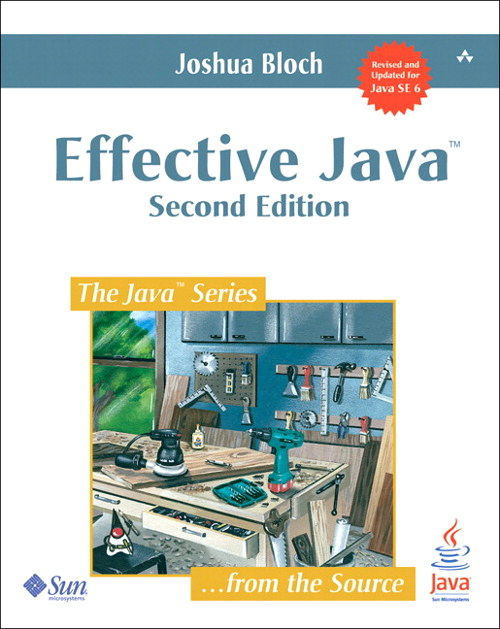
\includegraphics[width=5cm,height=6.3cm]{EJCover.png}
\end{center}
\end{frame}

\begin{frame}[fragile]
\frametitle{Homework}

\begin{itemize}[<+->]
	\item 1 Point
	\item Deadline: Nov. 13, Friday, 09:00
	\item Send the source code to\\
		abreslav@ut.ee
	\item Task:\\
		\begin{itemize}
		\item Write a class \texttt{Address}:
		\begin{itemize}
			\item Street
			\item Building
			\item Apartment
			\item Postal code
		\end{itemize}
		\item Define \texttt{equals} method to compare all fields.\\
		\item Write a utility method which takes a list of addresses and returns the number of different entries in this list.\\
		\item Write JUnit tests for your code.
		\end{itemize}
\end{itemize}

\end{frame}

\end{document}
